\problemname{Pingisturnering}
\noindent

Rulls är en äkta entusiast av PO (Pingisolympiaden).  
Han älskar att följa tävlingarna och heja på sina favoritspelare när de tävlar.

PO är en turnering i pingis med ett spännande format.  
Turneringen börjar med $N$ spelare, där varje spelare har en startposition.  
Baserat på startpositionerna möts spelarna parvis i matcher.  
Varje match resulterar i en vinnare och en förlorare.  
Förloraren blir eliminerad och spelar inga fler matcher,  
medan vinnaren går vidare för att möta vinnaren från en annan match.  
Processen upprepas tills endast en spelare återstår.

Turneringsformatet kan illustreras med ett träddiagram.

\begin{centering}
  \begin{figure}[h]
      \centering
      
\includegraphics[scale=0.7]{2.png}
    \caption{Bilden visar hur träddiagrammet av turneringsformatet ser ut för 4 personer. Placeringen av startpositionerna för spelarna är även en lösning för exempelfall 1.}
  \end{figure}
\end{centering}

Under den första omgången kommer spelaren på den första positionen att möta spelaren på den andra positionen, 
spelaren på den tredje positionen möter den fjärde, och så vidare. Vinnaren i varje par går vidare och kommer att paras ihop på samma sätt i nästa omgång.

För att organisatörerna inte ska behöva hantera jobbiga situationer garanteras det att antalet spelare alltid är en tvåpotens.

Nu är PO över för den här säsongen,  
men Rulls har glömt vilka matcher som spelats  
och vilka startpositioner varje spelare hade.  
Däremot minns han antalet matcher som varje spelare har vunnit.

Givet antalet vinster för de $N$ spelarna,  
skriv ut en möjlig ordning av startpositionerna för de $N$ spelarna.

Rulls minns även att startpositionerna var ordnade i den lexikografiskt minsta möjliga ordningen.
För att få full poäng krävs det att du hittar den lexikografiskt\footnote{https://sv.wikipedia.org/wiki/Lexikografisk\_ordning} minsta möjliga startpositionen.



En lösning $A$ är lexikografiskt mindre än en annan lösning $B$ om följande två villkor är uppfyllda:  
\begin{enumerate}  
    \item $A \neq B$.  
    \item Vid den första positionen där $A$ och $B$ har olika element, är elementet i $A$ mindre än elementet i $B$.  
\end{enumerate}  

Till exempel, om vi har två lösningar:  
$$
A = [1, 2, 4, 3], \quad B = [1, 3, 2, 4],  
$$  
så är den första positionen där $A$ och $B$ skiljer sig på position 1. Där har $A[1] = 2$ och $B[1] = 3$. Eftersom $2 < 3$, är $A$ lexikografiskt mindre än $B$.  


\section*{Indata}
Den första raden innehåller ett heltal $N$ ($1 \leq N \leq 2^{19}$), antalet spelare i turneringen. $N$ är garanterat att vara en tvåpotens.

Den andra raden innehåller $N$ heltal, där $a_i$ ($0 \leq a_i \leq 10^9$ för alla $1 \leq i \leq N$) är antalet matcher som den $i$:te pingisspelaren har vunnit under turneringen.

\section*{Utdata}
Skriv ut $N$ heltal, en permutation av heltalen $1,2,\ldots, N$, där permutationen representerar startpositionerna i turneringen. 
För att få fullpoäng krävs även att du skriver ut den lexikografiskt minsta permutationen.

Om det är omöjligt att hitta startpositioner för dessa $N$ spelare, skriv ut $-1$.

\section*{Poängsättning}
Din lösning kommer att testas på en mängd testfallsgrupper.
För att få poäng för en grupp så måste du klara alla testfall i gruppen.
För varje testgrupp, ifall ditt program svarar korrekt om det går eller inte, 
samt skriver ut en möjlig permutation som startposition, så får du \underline{\textbf{50\%}} av testgruppens poäng.

För att få alla poäng i en testgrupp behöver du skriva ut den lexikografiskt minsta permutationen.

\noindent
\begin{tabular}{| l | l | p{12cm} |}
  \hline
  \textbf{Grupp} & \textbf{Poäng} & \textbf{Gränser} \\ \hline
  $1$    & $2$        & $N \leq 2$ \\ \hline
  $2$    & $6$        & $N \leq 4$ \\ \hline
  $3$    & $12$       & $N \leq 8$ \\ \hline
  $4$    & $18$       & $N \leq 2^7 = 128$ \\ \hline
  $5$    & $12$       & $N \leq 2^{11} = 2048$ \\ \hline
  $6$    & $12$       & $a_i \leq a_{i+1}$ för alla $1 \leq i \leq N-1$. \\ \hline 
  $7$    & $38$       & Inga ytterligare begränsningar. \\ \hline % N <= 2^19 ≈ 5*10^5 eller 2^18 ≈ 2*10^5
\end{tabular}


\section*{Förklaring av exempelfall}
I första exempelfallet är en möjlig lösning att spelarna börjar i botten av turneringen enligt ordningen $[1, 3, 2, 4]$. Även om $[1, 4, 2, 3]$ också är en giltig lösning, så är den förstnämnda lösningen lexikografiskt mindre.
Notera att spelare $1$ kommer att köra en pingismatch mot spelare $3$, men eftersom vi vet att $3$ har förlorat alla sina matcher så måste $1$ ha vunnit den matchen.

\begin{centering}
  \begin{figure}[h]
      \centering
      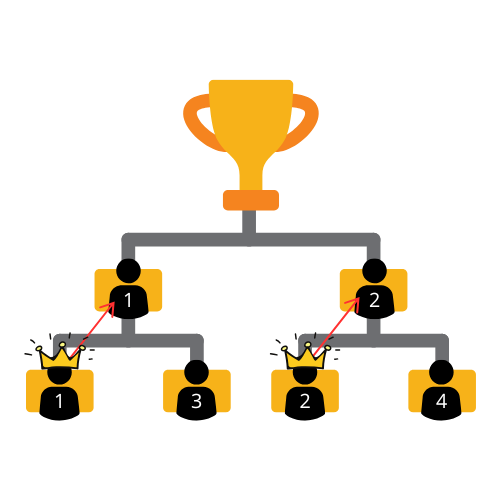
\includegraphics[scale=0.7]{4.png}
    \caption{Genom att placera spelarna enligt startpositionerna $[1, 3, 2, 4]$ i exempelfall 1, så vinner spelare 1 och spelare 2 sina första matcher.}
  \end{figure}
\end{centering}

\begin{centering}
  \begin{figure}[h]
      \centering
      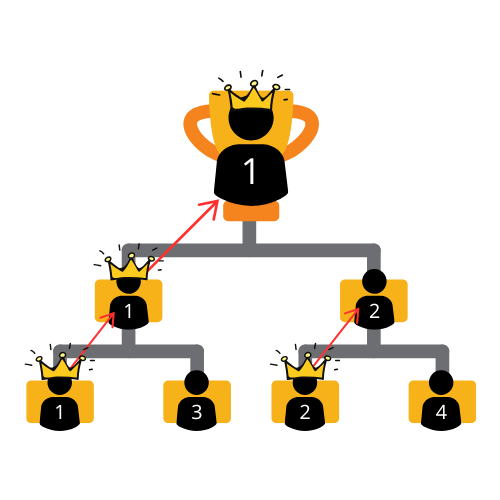
\includegraphics[scale=0.7]{6.png}
    \caption{Därefter vinner spelare 1 den sista matchen, vilket på så sätt uppfyller indatan.}
  \end{figure}
\end{centering}


I det andra exempelfallet är det omöjligt att alla spelar vinner 1 match. Därför skrivs ''-1'' ut.